%% AgentGuardUtil — CAR-bench Track 1 technical report (IJCAI-ECAI 2026 kit).
%% Build with the official IJCAI kit: place ijcai26.sty next to this file.
%% Falls back to a plain two-column layout when the kit is absent, so the
%% document always compiles for length checks.

\IfFileExists{ijcai26.sty}{%
  \documentclass{article}
  \pdfpagewidth=8.5in
  \pdfpageheight=11in
  \usepackage{ijcai26}
}{%
  \documentclass[twocolumn]{article}
  \usepackage[letterpaper,margin=0.75in,columnsep=0.25in]{geometry}
  \makeatletter
  \providecommand{\affiliations}[1]{\par\normalsize ##1}
  \providecommand{\emails}[1]{\par\texttt{\small ##1}}
  \makeatother
}
\usepackage{times}
\usepackage{amsmath,amssymb}
\usepackage{booktabs}
\usepackage{graphicx}
\usepackage{tikz}
\usetikzlibrary{arrows.meta,positioning}
\usepackage[ruled,vlined,linesnumbered]{algorithm2e}
\usepackage{url}

\newcommand{\pass}[1]{\ensuremath{\mathrm{Pass}^{#1}}}
\newcommand{\act}{\ensuremath{a}}
\newcommand{\hist}{\ensuremath{h}}

\title{From Policy Text to Executable Obligations:\\
A Grounded Verification Harness for Dependable In-Car LLM Agents}

\author{
Radouane Bouchekir
\and
Damir Safin
\and
Tomas Bueno Momcilovic
\affiliations
fortiss GmbH, Munich, Germany
\emails
\{bouchekir, safin, momcilovic\}@fortiss.org
}

\begin{document}
\maketitle

\begin{abstract}
Large language model (LLM) agents deployed in vehicles must satisfy a written
operating policy on every turn: a single hallucinated identifier, omitted
mandatory side-effect, or premature completion claim fails the task. We present
\emph{AgentGuardUtil}, our entry to CAR-bench Track~1, which treats the LLM as
a fallible proposer inside a grounded verify-and-revise loop. Its core novelty
is a \emph{runtime policy compiler}: the natural-language policy shipped with
each episode is compiled, once per policy, into typed machine-checkable rules,
a subset of which receive an \emph{executable} form. A deterministic obligation
engine interprets these rules against live tool results and the simulated
post-write state of the draft itself, emitting the exact remedial calls with
computed arguments rather than natural-language reminders. Around this engine,
${\sim}25$ deterministic gates (identifier provenance, schema and enum
validity, gather-before-act, confirmation and future-time protocols) and an LLM
critic produce tiered findings that drive a bounded revision loop tuned for the
$\pass{k}$ metric. Nothing is benchmark-specific: all checks derive from the
policy, tool schemas, and observations provided at run time.
\end{abstract}

\section{Introduction}
\paragraph{Context.}
LLM-based agents are moving rapidly from research prototypes into products
that act on the physical world. In-vehicle voice assistants are an exemplary
setting: the agent controls windows, climate, lighting, navigation, charging,
and communication on behalf of a driver whose attention is limited, under a
manufacturer policy that encodes safety and interaction rules. Here the cost
of an unreliable action --- a fabricated identifier, an omitted mandatory
side-effect, a confidently wrong ``done'' --- is not a benchmark point but a
trust and safety incident.

\paragraph{The problem.}
Existing agent benchmarks largely evaluate under idealized conditions ---
complete information, available tools, unambiguous instructions --- whereas
deployed agents face incomplete or ambiguous requests, capabilities that may
be missing, and domain policies that constrain behavior;
CAR-bench~\cite{carbench} was built around exactly this gap, and its baseline
studies report that frontier models systematically prioritize task completion
over admitting incapability. Concretely (Fig.~\ref{fig:overview}), a
simulated driver converses in closed loop with the agent, which observes and
mutates a vehicle--world environment through 58 tools under a multi-page
natural-language policy; tasks are scored on a \emph{conjunction} of criteria
(exact final \emph{and} intermediate environment states, tool coverage,
execution errors, automated and LLM-judged policy compliance, correct
termination), and the headline metric over $k$ repeated trials is
\begin{equation}
\pass{k} \;=\; \frac{1}{|\mathcal{T}|}\sum_{\tau\in\mathcal{T}}
\prod_{j=1}^{k}\mathbf{1}\!\left[\text{trial } j \text{ of } \tau \text{ passes}\right],
\label{eq:passk}
\end{equation}
with $k{=}3$ on the hidden test set. Under an i.i.d.\ Bernoulli model with
per-task success rate $q_\tau$,
$\mathbb{E}[\pass{k}]=\frac{1}{|\mathcal{T}|}\sum_\tau q_\tau^{\,k}$: the
metric is dominated by the \emph{stable core} of tasks with
$q_\tau\!\approx\!1$, while near-coin-flip tasks contribute almost nothing
($0.5^3{=}0.125$). The challenge is therefore twofold: suppress the
characteristic compliance failures (invented identifiers, skipped mandatory
side-effects, non-canonical write sequences, refusals of computable requests,
present-time answers to future-time constraints), and make correct behavior
\emph{repeatable} rather than merely likely.

\paragraph{Our approach.}
\emph{AgentGuardUtil} interposes a verification layer between the LLM and the
vehicle (Fig.~\ref{fig:overview}): the LLM only \emph{proposes}; a harness
grounded in the episode's own artifacts decides what may execute. At the
first turn, the natural-language policy is compiled --- once, and cached ---
into typed machine-checkable rules, part of which receive an
\emph{executable} form. On every draft action, a deterministic obligation
engine evaluates these rules against live tool results and the simulated
post-write state of the draft itself, computing the exact remedial calls the
policy requires; ${\sim}25$ further deterministic gates enforce identifier
provenance, schema validity, and interaction protocols, and an LLM critic
adjudicates the uncertain findings. Surviving findings drive a bounded
revise-and-recheck loop before anything reaches the environment. Our
contributions:
\begin{enumerate}
\itemsep0pt
\item a \textbf{runtime policy compiler} producing typed rules with an
executable sub-language, cached per policy hash (\S\ref{sec:compile});
\item a \textbf{deterministic obligation engine} that evaluates executable
rules on a projection of the environment state --- including \emph{simulation
of the draft's own writes} --- and emits exact remedial tool calls
(\S\ref{sec:oblig});
\item a \textbf{tiered verification loop} combining deterministic gates with
an LLM critic, engineered for $\pass{k}$ stability (\S\ref{sec:verify});
\item an \textbf{empirical variance analysis} on the public splits motivating
these choices (\S\ref{sec:eval}).
\end{enumerate}
The design composes chain-of-verification
prompting~\cite{dhuliawala2023cove}, self-consistency~\cite{wang2023sc}, and
tool-use agent patterns~\cite{yao2023react,yao2024tau}, but moves the
decisive checks out of the model and into code that the model cannot
hallucinate around.

\begin{figure}[t]
\centering
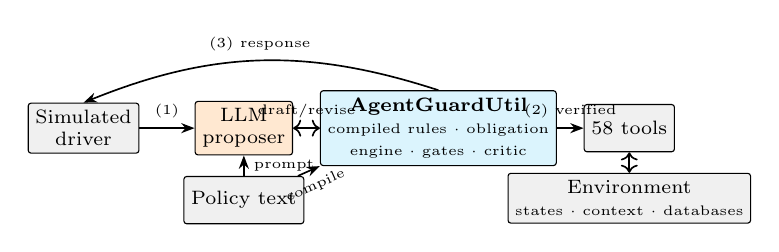
\begin{tikzpicture}[
  font=\scriptsize,
  node distance=3mm and 3.4mm,
  box/.style={draw,rounded corners=1pt,align=center,inner sep=2.6pt,minimum height=6mm},
  llm/.style={box,fill=orange!18},
  det/.style={box,fill=cyan!14},
  env/.style={box,fill=gray!12},
  arr/.style={-{Stealth[length=1.7mm]},semithick}
]
\node[env] (user) {Simulated\\driver};
\node[llm,right=7mm of user] (agent) {LLM\\proposer};
\node[det,right=of agent] (harness) {\textbf{AgentGuardUtil}\\ \tiny compiled rules $\cdot$ obligation\\ \tiny engine $\cdot$ gates $\cdot$ critic};
\node[env,right=of harness] (tools) {58 tools};
\node[env,below=2.6mm of tools] (world) {Environment\\ \tiny states $\cdot$ context $\cdot$ databases};
\node[env,below=2.6mm of agent] (policy) {Policy text};
\draw[arr] (user) -- node[above]{\tiny (1)} (agent);
\draw[arr,<->] (agent) -- node[above]{\tiny draft/revise} (harness);
\draw[arr] (harness) -- node[above]{\tiny (2) verified} (tools);
\draw[arr,<->] (tools) -- (world);
\draw[arr] (policy) -- node[below,sloped]{\tiny compile} (harness.south west);
\draw[arr] (policy) -- node[right]{\tiny prompt} (agent);
\draw[arr] (harness.north) to[bend right=20] node[above]{\tiny (3) response} (user.north);
\end{tikzpicture}
\caption{AgentGuardUtil in the CAR-bench loop~\cite{carbench}: the simulated
driver (1) converses with the agent; the LLM only drafts, the harness
verifies and revises before (2) tool execution against the vehicle--world
environment and (3) the spoken response. The policy is both the LLM's prompt
and the harness's compilation source.}
\label{fig:overview}
\end{figure}

\begin{figure}[t]
\centering
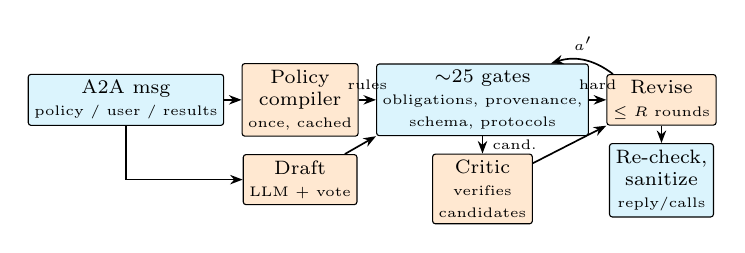
\begin{tikzpicture}[
  font=\scriptsize,
  node distance=2.2mm and 2.2mm,
  box/.style={draw,rounded corners=1pt,align=center,inner sep=2.2pt,minimum height=5.5mm},
  llm/.style={box,fill=orange!18},
  det/.style={box,fill=cyan!14},
  arr/.style={-{Stealth[length=1.6mm]},semithick}
]
\node[det]  (msg)  {A2A msg\\ \tiny policy / user / results};
\node[llm,right=of msg] (comp) {Policy\\compiler\\ \tiny once, cached};
\node[llm,below=of comp] (draft) {Draft\\ \tiny LLM + vote};
\node[det,right=of comp] (gates) {$\sim$25 gates\\ \tiny obligations, provenance,\\ \tiny schema, protocols};
\node[llm,below=of gates] (critic) {Critic\\ \tiny verifies\\ \tiny candidates};
\node[llm,right=of gates] (rev) {Revise\\ \tiny $\le R$ rounds};
\node[det,below=of rev] (out) {Re-check,\\sanitize\\ \tiny reply/calls};
\draw[arr] (msg) -- (comp);
\draw[arr] (msg.south) |- (draft.west);
\draw[arr] (comp) -- node[above]{\tiny rules} (gates);
\draw[arr] (draft) -- (gates.south west);
\draw[arr] (gates) -- node[right]{\tiny cand.} (critic);
\draw[arr] (gates) -- node[above]{\tiny hard} (rev);
\draw[arr] (critic) -- (rev.south west);
\draw[arr] (rev) to[bend right=28] node[above]{\tiny $a'$} (gates);
\draw[arr] (rev) -- (out);
\end{tikzpicture}
\caption{One agent turn. Orange components call an LLM; cyan components are
deterministic. The compiler runs once per distinct policy; the gate suite and
obligation engine run on every draft.}
\label{fig:pipeline}
\end{figure}

\section{The AgentGuardUtil Harness}

\subsection{Turn Pipeline}
Figure~\ref{fig:pipeline} and Algorithm~\ref{alg:turn} summarize one turn. The
student LLM proposes a draft action $\act$ (a spoken reply and/or tool calls)
given the history $\hist$ and tool schemas $\mathcal{S}$. When the draft
mutates state and voting is enabled, $n$ samples are drawn and the modal
\emph{action set} (order-insensitive multiset of normalized calls) is kept ---
self-consistency applied only where errors are irreversible. The draft then
enters verification (\S\ref{sec:verify}); surviving findings are injected as an
internal note and the model revises, for at most $R$ rounds ($R{=}2$).
Because a revision may itself introduce a new defect, a final
deterministic-only re-check runs once, optionally with a stronger
\emph{escalation} model. A text sanitizer strips non-speakable markup, and
A2A \texttt{turn\_metrics} (token usage, cost, latency across \emph{all}
internal calls) are attached to turn-final responses.

\begin{algorithm}[t]
\caption{\textsc{VerifiedTurn}$(\hist,\mathcal{S})$}
\label{alg:turn}
\scriptsize
\If{first turn for this policy $\Pi$}{
  $\mathcal{R}\leftarrow\textsc{Compile}(\Pi,\mathcal{S})$ \tcp*{cached by $\mathrm{hash}(\Pi)$}}
$L \leftarrow L \cup \textsc{ExtractAsks}(\text{new user msg})$\;
$\act\leftarrow\textsc{ModalVote}\big(\{\textsc{LLM}(\hist,\mathcal{S})\}_{1..n}\big)$\;
\For{$i\leftarrow 1$ \KwTo $R$}{
  $F \leftarrow F_{\mathrm{hard}}(\act,\hist,\mathcal{R})
        \,\cup\, \textsc{Critic}\big(F_{\mathrm{adv}}(\act,\hist,\mathcal{R})\big)$\;
  \lIf{$F=\emptyset$}{\textbf{break}}
  $\act\leftarrow\textsc{Revise}(\hist,\act,F)$\;
}
\If{$\act$ was revised \textbf{and} $F_{\mathrm{hard}}(\act)\neq\emptyset$}{
  $\act\leftarrow\textsc{Revise}_{\mathrm{esc}}(\hist,\act,F_{\mathrm{hard}}(\act))$
  \tcp*{safety net}}
\Return{$\textsc{Sanitize}(\act)$}
\end{algorithm}

\subsection{Runtime Policy Compilation}
\label{sec:compile}
At the first turn of an episode the policy text $\Pi$ (with volatile
location/time fields normalized out) is compiled by an LLM into a rule set
$\mathcal{R}$, cached process-wide under $\mathrm{hash}(\Pi)$ so compilation
adds no per-task variance. Each rule
$r=\langle \mathrm{id},\,\kappa,\,\mathcal{T}_r,\,\rho\rangle$ carries a type
$\kappa$ (\emph{precondition, auto-action, confirmation, prohibition,
disclosure, constraint, selection}), trigger tools $\mathcal{T}_r$ grounded
against the live tool inventory, and an imperative requirement $\rho$.
Compound clauses are split into atomic rules (one condition, one remedy). A
second, focused pass translates state-conditional rules into an
\emph{executable} form
\begin{equation}
e_r=\big\langle g,\;\varphi,\;\lhd,\;v,\;\omega \big\rangle,
\label{eq:exec}
\end{equation}
where $g$ is a read tool, $\varphi$ a field-name pattern with one wildcard,
$\lhd\in\{<,\le,>,\ge,=,\ne,\ni,\not\ni\}$, $v$ a threshold, and
$\omega(x)=\langle u,\beta(x)\rangle$ an obligation template binding the
matched item $x$ into the arguments of tool $u$, validated against the
declared enum of $u$'s schema. The compiler sees real signatures
$u(p_1,\dots,p_m)$; an obligation whose arguments cannot be validated is
dropped, degrading that rule to advisory --- the engine can only \emph{add}
precision, never force an invalid call.

\subsection{Executable Obligations}
\label{sec:oblig}
Let $\sigma_g$ be the latest parsed result of read $g$ and
$w_1,\dots,w_m$ the write calls executed after it, followed by the draft's own
writes $W_\act$. The engine forms a \emph{projected} state
$\hat{\sigma}=\pi(\sigma_g;\,w_{1..m}\!\cdot\!W_\act)$: a write matching some
obligation template is \emph{simulated} (the addressed fields are assigned the
written value, with \texttt{ALL}-style enum members fanning out over all
matching fields); a write that merely shares the field's subject tokens
\emph{invalidates} only those fields; a write whose tool result reports an
error invalidates rather than simulates. Evaluating conditions on the
\emph{post-write} projection is what lets a draft that itself creates a
violation (e.g.\ opening all windows to 50\% while the air conditioning is on)
generate its own remediation. The computed obligation set is
\begin{equation}
\Omega(\act,\hist)=
\bigcup_{r\in\mathcal{R}_{\triangleright}}
\big\{\omega(x)\;:\;\varphi\!\sim\!x,\ \hat{\sigma}(x)\lhd v\big\}
\;\setminus\;\big(E_\hist\cup A_\act\big),
\label{eq:oblig}
\end{equation}
where $\mathcal{R}_{\triangleright}=\{r:\mathcal{T}_r\cap(W_\hist\cup
W_\act)\neq\emptyset\}$ are the triggered rules; obligations whose condition
holds on $\hat{\sigma}$ survive, minus calls already executed ($E_\hist$) or
contained in the draft ($A_\act$). When every matched item qualifies with identical residual
arguments and the schema declares an \texttt{ALL}-style member, the set is
collapsed to a single aggregate call --- matching the canonical action
granularity that intermediate-state scoring expects. Symmetric checks flag
\emph{excess}: writes on items the condition exempts, and aggregate calls
where only a subset qualifies. Findings quote ready-to-execute calls with
evidence (``\texttt{window\_driver\_position}$=25>20$''), turning policy
compliance from recall into transcription.

\subsection{Tiered Verification and Variance Control}
\label{sec:verify}
Around the obligation engine run ${\sim}25$ deterministic gates, including:
\emph{identifier provenance} (every opaque id in outgoing arguments must
appear in prior observations --- a deterministic anti-hallucination oracle);
\emph{schema/enum validity} pre-execution; \emph{gather-before-act} and
preference-retrieval requirements; a \emph{confirmation protocol} gate
(confirmation-marked tools blocked until an intent question was affirmed);
\emph{completion} and \emph{plan-completion} gates (no success claims without
matching actions); a \emph{refusal-read} gate (a can't-do reply without ever
reading the relevant subsystem must first perform the free read); and a
\emph{future-condition} gate (requests referencing arrival times or future
windows must not be answered with current-moment filters, but by fetching
unfiltered data and evaluating the constraint from returned fields).

Findings are \emph{tiered}: hard findings (deterministically certain) always
trigger revision; advisory candidates are passed to an LLM critic that
verifies them against the transcript and tool schemas, and only confirmed
items survive~\cite{dhuliawala2023cove}. This tiering is a variance mechanism:
under Eq.~\eqref{eq:passk} a spurious revision on a correct draft is as costly
as a missed defect, so uncertain signals must not force edits. Two further
mechanisms serve $\pass{k}$: revision is \emph{bounded} with an oscillation
valve (a write-set once revised away and re-proposed relaxes the gather gate
instead of looping), and every layer is fail-safe (an internal exception
contributes no findings rather than crashing the turn).

\section{Generalization and Deployment}
No gate, rule, tool name, or threshold is benchmark-specific: everything is
derived at run time from the provided policy, tool schemas, and observations,
so the harness transfers unchanged to the hidden set --- and beyond it (unit
tests include alien-domain policies such as smart-home and greenhouse
control). The agent ships as a digest-pinned \texttt{linux/amd64} image; every
layer is switchable via \texttt{ENABLE\_*} environment flags, and model,
provider route, and sampling are env-configurable (LiteLLM). The submission
configuration runs Claude Opus~4.8 via the direct Anthropic API and was
validated end-to-end with the official evaluator image (GHCR option-C
protocol). The code base carries 108 deterministic unit tests and structured
per-turn traces (drafts, fired gates, findings) for auditability.

\section{Empirical Analysis}
\label{sec:eval}
\begin{table}[t]
\centering
\scriptsize
\begin{tabular}{lccc}
\toprule
Public split & Tasks & $\pass{1}$ & Cost/task \\
\midrule
Base & 50 & 74.0\% & \$0.054 \\
Hallucination & 48 & 62.5\% & \$0.039 \\
Disambiguation (3 runs) & 31 & 48.4--58.1\% & \$0.073--0.085 \\
\bottomrule
\end{tabular}
\caption{Development results on the public training splits with a
\texttt{gemini-2.5-flash} student in all harness roles (best base run;
disambiguation shown as min--max over three full runs). The submitted
configuration upgrades the student to Claude Opus~4.8.}
\label{tab:results}
\end{table}

Table~\ref{tab:results} reports development results with a deliberately weak
and inexpensive student model, chosen to stress the harness rather than the
LLM. The most consequential measurement is \emph{run-to-run variance}: across
repeated identical disambiguation runs, 42--44\% of tasks flipped outcome at
least once, and two same-configuration runs agreed on only $25/31$ tasks. In
the Bernoulli view of Eq.~\eqref{eq:passk} this places a large task mass at
intermediate $q_\tau$, where the $k{=}3$ product annihilates score --- e.g.\
the stable-pass core across three disambiguation runs was $9/31$ tasks,
against single-run $\pass{1}$ of ${\sim}52\%$. Failure forensics against
ground-truth action chains attribute the residual gap to model-reasoning
classes --- guessed unstated argument values, arrival-time constraints
answered with current-state reads, and non-canonical write granularity
breaking intermediate-state subsets --- each of which motivated a dedicated
generic gate (\S\ref{sec:verify}); harness interventions themselves are
verified regression-safe by construction (read-only remedies, conjunctive
trigger conditions). These diagnostics, and the leaderboard dominance of
stronger students on identical scaffolds, drove the submission choice of a
frontier student model with the verification budget concentrated on
deterministic, zero-variance checks.

\section{Conclusion}
AgentGuardUtil demonstrates that the reliability demands of in-vehicle
assistants are best met not by prompting alone but by \emph{compiling} the
operating policy into executable obligations and letting deterministic code
--- grounded in live observations and simulated post-write state --- decide
what the model must do, verify, or refrain from. The design is
benchmark-agnostic by construction and engineered for the repeatability that
$\pass{k}$ rewards.

\paragraph{Code.} \url{https://github.com/BouchekirRedouane/car-bench-ijcai}

\begin{thebibliography}{7}
\scriptsize
\bibitem{carbench}
CAR-bench: Car Assistant Reliability Benchmark. IJCAI-ECAI 2026 Competition,
Track~1. \url{https://car-bench.github.io/car-bench/}, 2026.

\bibitem{dhuliawala2023cove}
S.~Dhuliawala, M.~Komeili, J.~Xu, R.~Raileanu, X.~Li, A.~Celikyilmaz, and
J.~Weston. Chain-of-verification reduces hallucination in large language
models. \emph{arXiv:2309.11495}, 2023.

\bibitem{wang2023sc}
X.~Wang, J.~Wei, D.~Schuurmans, Q.~Le, E.~Chi, S.~Narang, A.~Chowdhery, and
D.~Zhou. Self-consistency improves chain of thought reasoning in language
models. In \emph{ICLR}, 2023.

\bibitem{yao2023react}
S.~Yao, J.~Zhao, D.~Yu, N.~Du, I.~Shafran, K.~Narasimhan, and Y.~Cao. ReAct:
Synergizing reasoning and acting in language models. In \emph{ICLR}, 2023.

\bibitem{yao2024tau}
S.~Yao, N.~Shinn, P.~Razavi, and K.~Narasimhan. $\tau$-bench: A benchmark for
tool-agent-user interaction in real-world domains. \emph{arXiv:2406.12045},
2024.
\end{thebibliography}

\end{document}
